\section{OPCUA - Semantik}\label{ch:opcua}

\begin{figure*}[thpb]
      \centering
      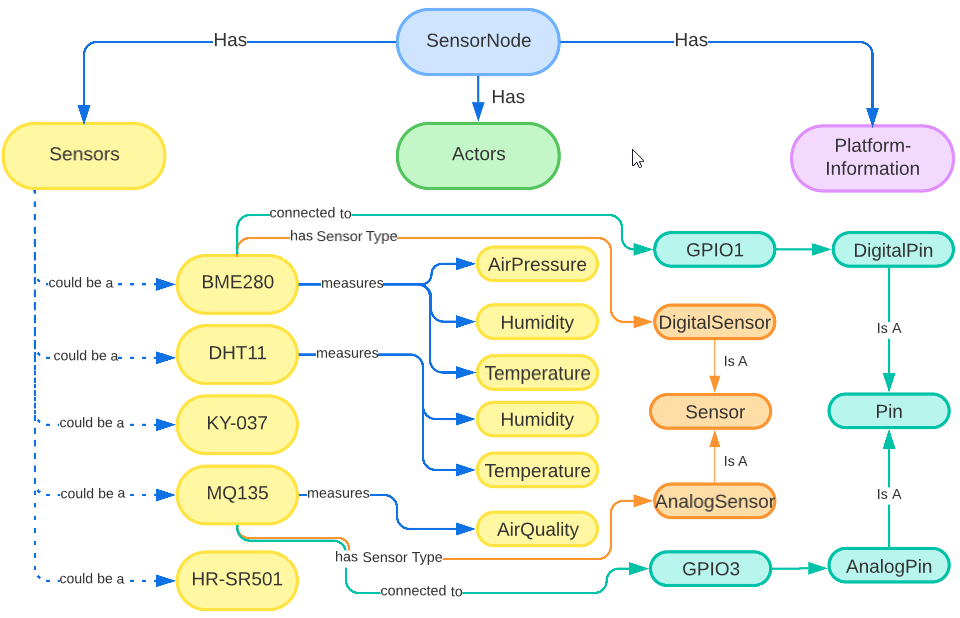
\includegraphics[scale=0.4]{abbildungen/opcua_semantic_schema.png}
      \caption{Beispiel Semantisches Modell Sensornetzwerk}
\end{figure*}
Basis eines OPCUA Server ist ein sog. Informationsmodell (Semantisches Modell), welches die zu einem Anwendungsfall vorliegenden Informationen gliedert. Analog zur Automatisierungspyramide werden die Informationen zunächst hierarchisch in einer Baumstruktur gegliedert. Ergänzt wird das Informationsmodell durch nicht hierarchische Verbindungen zwischen den Knoten, damit auch komplexere Sachverhalte abgebildet werden können.
\newline
\newline
Durch die Verbindung zweier Knoten mit einer entsprechenden Referenz entsteht eine semantische Bedeutung. So stellt beispielsweise die Verbindung „BME280 – measures - Temperature“, analog zu anderen semantischen Beschreibungen eine Verbindung von Subjekt, Prädikat und Objekt dar.
Um z.B. alle Sensoren zu finden, die die Temperatur messen können, wird nach nach allen Verbindungen mit Subjekt x, die nach dem Schema „x – measures – Temperature“ aufgebaut sind gesucht, was in dem Modell in Abbildung 1 die zwei Knoten BME280 und DHT11 zurückliefern würde.
\newline
\newline
Durch das Festlegen von semantischen Regeln kann ein erstelltes Informationsmodell validiert werden. So kann beispielsweise festgelegt werden, dass in dem Beispiel aus Abbildung 1 ein Sensor mit Sensor Type „Digital Sensor“ keine „Connected To“-Referenz auf einen GPIO-Pin aufweisen darf, der vom Typ „AnalogPin“ ist.
\newline
\begin{lstlisting}[caption={Semantische Validierung Digitaler Sensor},captionpos=b,showstringspaces=false, basicstyle=\footnotesize]
IF x - has Sensor Type - DigitalSensor
AND x - connected to - y - has Pin Type - AnalogPin: 
    VALIDATION = FALSE
\end{lstlisting}

Im vorliegenden Anwendungsfall heißt dies praktisch, dass ein Sensor, der ein digitales Signal ausgibt, nicht an einen Pin des Raspberry Pis angeschlossen werden darf, der nur für Analoge Signale geeignet ist. 
